\section{Constitutive equations - Materials}
\label{sec:constitutive_equations_materials}

Constitutive relationships are necessary to specify the properties for fluid flow, heat transfer, swelling pressure and mechanical stress/deformation of the specific material under consideration. For determination of material properties laboratory tests have to be conducted. A number of material properties can not be determined directly.
This must be done by back analysis using inverse modeling.

For THM processes we have to consider 
hydraulic
(Section \ref{sec:h_properties}),
thermal,
(Section \ref{sec:t_properties})
and
mechanical properties
(Section \ref{sec:m_properties})
of the corresponding fluid and solid phases.

% Hydraulic properties
\subsection{Hydraulic properties}
\label{sec:h_properties}

Recalling the balance equations for fluid mass (\ref{eqn:mass_pormed_deform}) and fluid momentum (\ref{eqn:momentum_balance_fluid}), i.e. Darcy's law the following material quantities needs to be specified: fluid densities $\rho^\Phase$, fluid viscosities $\mu^\Phase$, permeabilities $\PermRelP^{\gamma}, \PermTensor$, and porosity $n$.
Fluid phase pressures $p^\Phase$, saturations $S^\Phase$ and velocities $\VelocityVector^{\Phase s}$ are considered state variables.

%-------------------------------------------------------------------------
\subsubsection{Density - $\rho$}

Density is considered as a mechanical material property (sec. \ref{sec:m_properties}).

%-------------------------------------------------------------------------
\subsubsection{Viscosity - $\Viscosity^\Phase$}

Viscosity is defined as shearing stress per unit area divided by a
velocity gradient and it has the dimension of $N\,s/m^2$ or
$Pa\,s$.

\begin{figure}[htb!]
\begin{center}
\footnotesize
\includegraphics[width=0.75\columnwidth]{chapter20/figures/visco9.eps}
\caption{Water viscosity as a function of temperature}
\label{fig:visco9}
\end{center}
\end{figure}

\begin{itemize}
%.........................................................................
 \item
Non-isothermal flow of water (de Marsily 1986) (Fig. \ref{fig:visco9})
\begin{eqnarray}
\Viscosity^w (\Temperature)
=
2.285 \times 10^{-5}
+
1.01 \times 10^{-3} \log\Temperature
\end{eqnarray}
%.........................................................................
\item
Non-isothermal flow of gas (Reid et al. 1988)
(Fig. \ref{fig:visco7})
\begin{eqnarray}
\Viscosity^g (\Pressure,\Temperature)
=
\Viscosity_0
\left(
1 + \frac{A\Pressure_r^{3/2}}{B\Pressure_r+(1+C\Pressure_r^D)^{-1}}
\right)
\end{eqnarray}
%
with the following parameters:
\begin{eqnarray}
\begin{array}{ll}
\Pressure_r = \Pressure / \Pressure_{\mbox{\footnotesize crit}}
&
\Temperature_r = \Temperature / \Temperature_{\mbox{\footnotesize crit}}
\\
A = \D\frac{\alpha_1}{T_r} \exp (\alpha_2 T_r^a)
&
B = A(\beta_1 T_r - \beta_2)
\\
C = \D\frac{\gamma_1}{T_r} \exp (\gamma_2 T_r^c)
&
D = \D\frac{\delta_1}{T_r} \exp (\delta_2 T_r^d)
\end{array}
\\
\begin{array}{lll}
\Pressure_{\mbox{\footnotesize crit}} = 33.9 \times 10^4 \, Pa
&
\Temperature_{\mbox{\footnotesize crit}} = 126.2 \, K
\\
\alpha_1 = 1.9824\times 10^{-3}  &  \alpha_2 = 5.2683  &  a = -0.5767 \\
\beta_1  = 1.65552               &  \beta_2  = 1.2760  &  \\
\gamma_1 = 0.1319                &  \gamma_2 = 3.7035  &  c = -79.8678 \\
\delta_1 = 2.9496                &  \delta_2 = 2.9190  &  d = -16.6169
\end{array}
\nonumber
\end{eqnarray}

\begin{figure}[htb!]
\begin{center}
\footnotesize
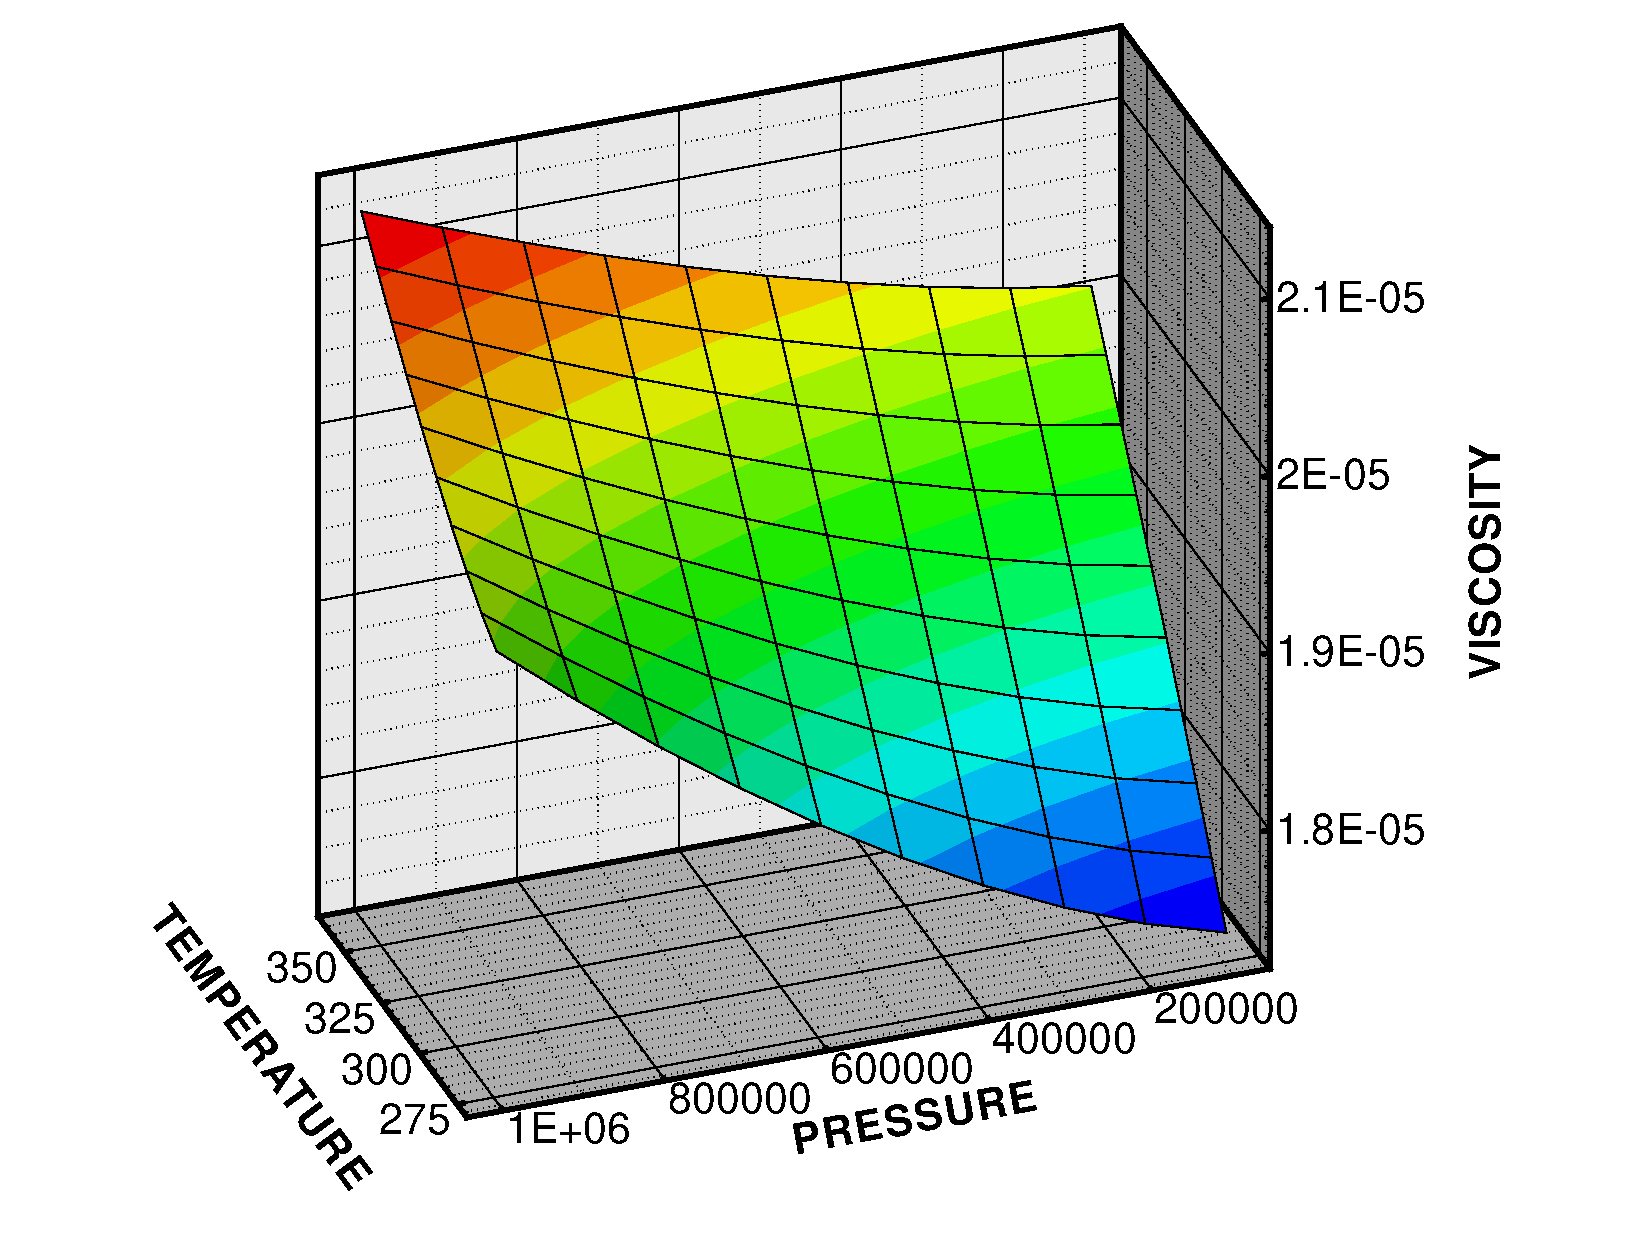
\includegraphics[width=0.6\columnwidth]{chapter20/figures/viscosity.eps}  % Filename.eps
\caption{Gas viscosity as a function of temperature and pressure}
\label{fig:visco7}
\end{center}
\end{figure}
%

\item
Non-isothermal flow of brines
(Lever and Jackson 1985)
\begin{eqnarray}
\Viscosity^w (\Temperature,\Conc)
=
\Viscosity_0
\frac{1+1.85\omega-4.1\omega^2+44.5\omega^3}{1+0.7063\zeta-0.04832\zeta^2}
\end{eqnarray}
with:
\begin{eqnarray}
\omega = \frac{\Conc}{\Density}
\quad , \quad
\zeta = \frac{T-150�C}{100�C}
\end{eqnarray}

\end{itemize}


%-------------------------------------------------------------------
\subsubsection*{Relative permeability - $\PermRelP^\Phase(\Saturation^\Phase)$}

For porous media containing more than one fluid, the concept of
relative permeability is introduced.  The relative permeability is
used to calculate the effective permeability
$(\PermRelP^\Phase\Saturation^\Phase)\PermTensor$, which is
described in the extended Darcy law.  The relationship depends
strongly on the saturations. Different relationships are possible:
constant values, user-defined functions, linear functions,
potential functions, or functions found in literature, such as the
van Genuchten Model (1980)
\begin{eqnarray}
\PermRelS(\Saturation^l)
=
\SaturationEff^{1/2}
\left(
1-(1-\SaturationEff^{1/\beta})^\beta
\right)^2
\label{eqn:relative_permeability_saturation}
\end{eqnarray}

$\PermTensor$ is the permeability of fully liquid saturated porous medium, i.e. the maximum permeability for liquid flow.
%
Capillary pressure and relative permeabilities are among
the most important parameters affecting multi-phase flow.

\begin{figure}[htb!]
\begin{center}
\footnotesize
\includegraphics[width=0.49\columnwidth]{chapter20/figures/persat.eps}  % Filename.eps
\includegraphics[width=0.49\columnwidth]{chapter20/figures/capsat.eps}  % Filename.eps
\caption{Relative permeability (left) and capillary pressure (right) as functions of liquid saturation for two different porous media: crystalline rock and bentonite}
\label{fig:capillarity}
\end{center}
\end{figure}

%-------------------------------------------------------------------
\subsubsection*{Capillary pressure - $\CapillaryPressure(\Saturation)$}

The capillary pressure can be defined as the tendency of a porous
medium to suck in the wetting fluid phase or to repel the
non-wetting phase.  Capillary pressure results from the pressure
discontinuity at the interface between two immiscible fluids.
Capillary pressure depends on the geometry of the void space, on
the nature of solids and liquids and on the degree of saturation.
In porous media the geometry of the void space is idealized. Thus,
the dependence reduces to saturation for any given porous media.
Care has to be taken, as capillary pressure is not the same for
drainage and re-wetting. The function connecting capillary
pressure and saturation has to be determined by laboratory
experiments for every new porous medium.
Frequently, an analytical
functions is used, such as the van Genuchten (1980) model
%
\begin{eqnarray}
\CapillaryPressure(\Saturation^l)
=
\left\{
\begin{array}{ll}
0 & \Saturation^l > \SaturationMax^l
\\
\frac{\Density^l g}{\alpha} (\SaturationEff^{-1/m}-1)^{1/n} &
\SaturationRes^l < \Saturation^l < \SaturationMax^l
\\
\CapillaryPressureMax & \Saturation^l < \SaturationRes^l
\end{array}
\right.
\label{eqn:capillary_pressure_saturation}
\end{eqnarray}

whit the effective saturation
\begin{eqnarray}
\SaturationEff
=
\frac{\Saturation^l - \SaturationRes^l}{1-\SaturationRes^l}
=
\left( 1 + (\alpha \, \CapillaryPressure)^n \right)^m
\qquad , \qquad \CapillaryPressure > 0
\end{eqnarray}



% Thermal properties
\subsection{Thermal properties}
\label{sec:t_properties}

Thermal properties we have to consider are heat capacity $\HeatCapacity$ and thermal conductivity $\lambda$.
In the following we introduce the properties for gases and liquids separately.

%.........................................................................
\subsubsection{Specific heat capacity - $\HeatCapacity$}

Specific heat capacity is defined by the equations.
%
\begin{eqnarray}
\HeatCapacity_V
=
\frac{\p e}{\p\Temperature}
\quad , \quad
\HeatCapacity_p
=
\frac{\p\Enthalpy}{\p\Temperature}
\equiv
c
\end{eqnarray}

Therefore, specific enthalpy can be calculated from following relation.
%
\begin{eqnarray}
\Enthalpy(\Temperature)
=
\int_{T_0}^{T}
\HeatCapacity_p
d\theta
\end{eqnarray}

Heat capacity $c\rho$ of the composite porous medium
contains contributions of all involved phases.

\begin{eqnarray}
c\rho
=
(1-n)c^s\rho^s
+
\sum_\Phase S^\Phase c^\Phase \rho^\Phase
\label{eqn:heat_capacity}
\end{eqnarray}

%.........................................................................
\subsubsection{Thermal conductivity - $\lambda$}

Concuctive heat flux is assumed to be governed by Fourier's law
%
\begin{eqnarray}
\Flux_T
=
- 
\HeatConductivity(\Saturation,\Porosity)
\nabla\Temperature
\end{eqnarray}
%
where $\HeatConductivity$ is the overall thermal conductivity of the porous medium. Overall thermal conductivity depends on porosity and saturation and is given by a geometric mean approximation.
%

Thermal conductivity $\lambda$ of the composite porous medium
contains contributions of all involved phases.

\begin{itemize}
	\item Geometric mean
\begin{eqnarray}
\HeatConductivity
=
(\HeatConductivity^s)^{(1-\Porosity)}
\prod_\Phase
(\HeatConductivity^\Phase)^{\Porosity\Saturation^\Phase}
\end{eqnarray}

	\item Arithmetric mean
\begin{eqnarray}
\HeatConductivity
=
(1-n)\HeatConductivity^s
+
\sum_\Phase S^\Phase \HeatConductivity^\Phase
\label{eqn:thermal_conductivity}
\end{eqnarray}

\end{itemize}

%.........................................................................
\subsubsection{Gases}

Beside the hydraulic characteristics such as air viscosity, the thermal gas and solid properties such as heat capacity and thermal conductivity are important for heat transport.
As an example, Fig. \ref{fig:thermal_properties} depicts the thermal properties of the gaseous phase.
Fig. \ref{fig:thermal_properties} (left) shows the temperature dependence of specific heat capacity of air at atmospheric pressure corresponding to equation (\ref{eqn:heat_capacity}) from \cite{ZografosEtAl:1987} compared with experimental data by \cite{VargaftikEtAl:1996}. Fig. \ref{fig:thermal_properties} (right) illustrates the temperature dependence of thermal conductivity of air at atmospheric pressure corresponding to equation (\ref{eqn:thermal_conductivity}) from \cite{ZografosEtAl:1987} compared with experimental data by \cite{VargaftikEtAl:1996}. The pressure dependency of thermal properties can be neglected in the present pressure regimes.

\begin{eqnarray}
c^g
=
1.0613
&-&
4.3282 \times 10^{-4} T
\nonumber\\
&+&
1.0234 \times 10^{-6} T^2
\nonumber\\
&-&
6.4747 \times 10^{-10} T^3
\nonumber\\
&+&
1.3864 \times 10^{-13} T^4
\label{eqn:heat_capacity}
\end{eqnarray}

\begin{eqnarray}
\lambda^g
=
7.488 \times 10^{-3}
&-&
1.7082 \times 10^{-4} T
\nonumber\\
&+&
2.3758 \times 10^{-7} T^2
\nonumber\\
&-&
2.2012 \times 10^{-10} T^3
\nonumber\\
&+&
9.46 \times 10^{-14} T^4
\nonumber\\
&-&
1.579 \times 10^{-17} T^5
\label{eqn:thermal_conductivity}
\end{eqnarray}

\begin{figure}[htb!]
\begin{center}
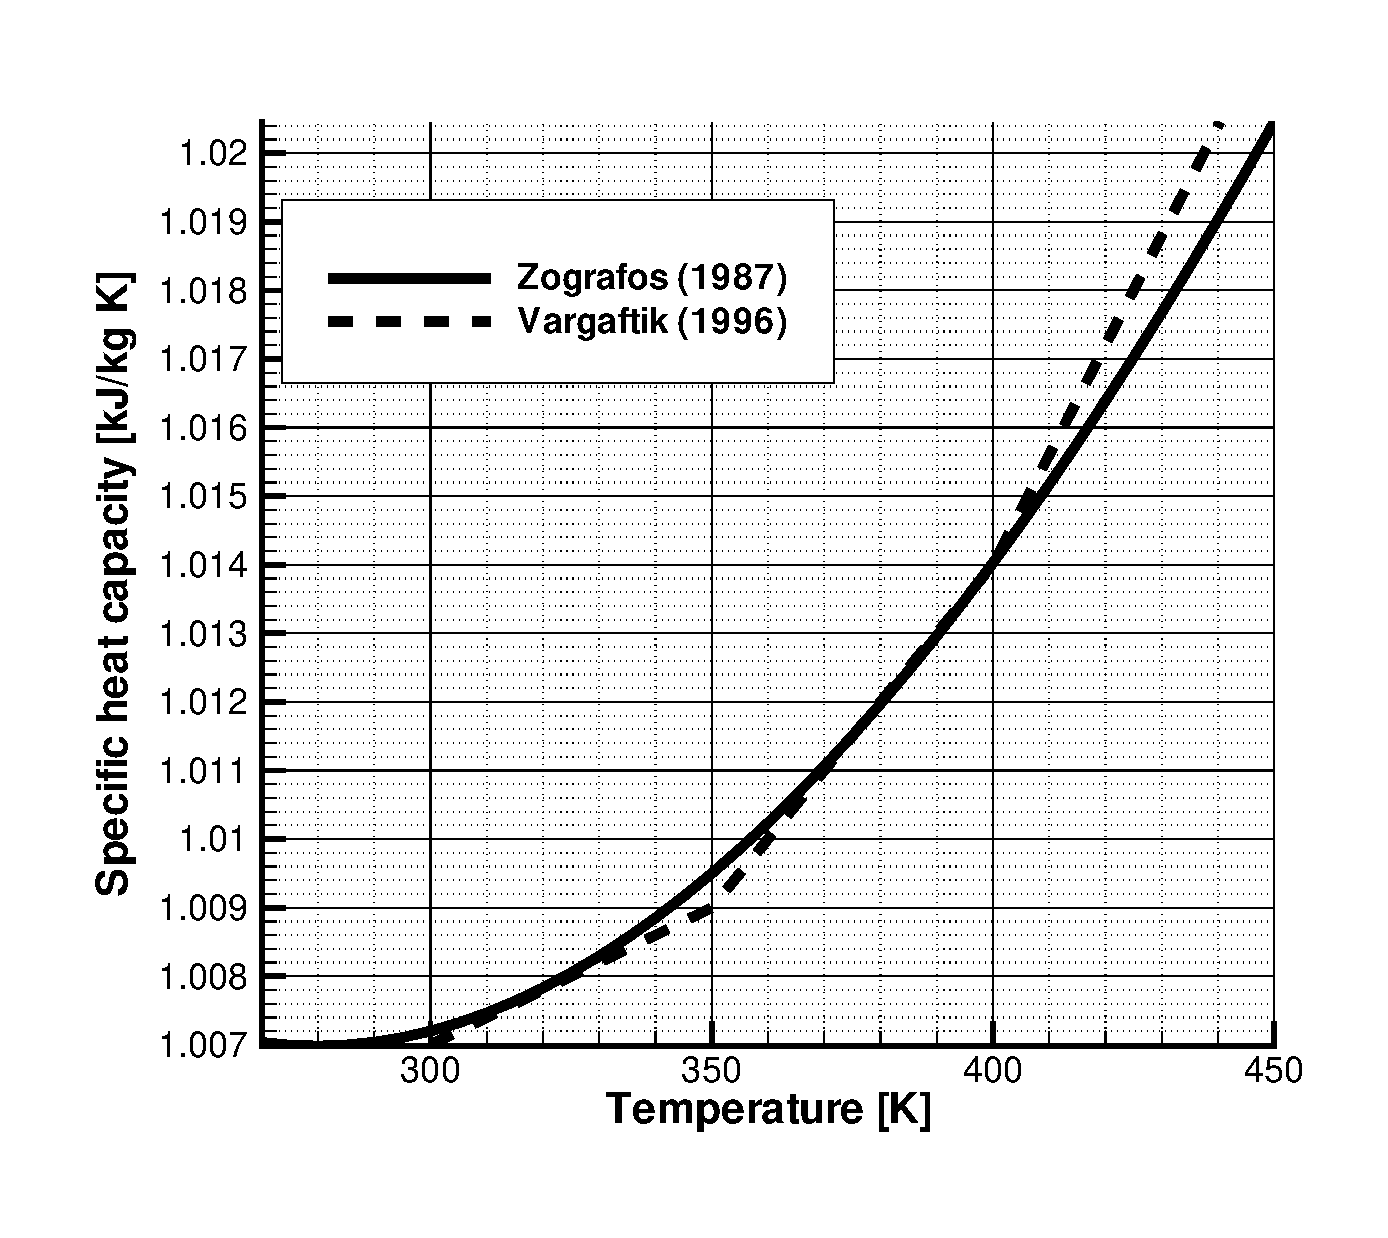
\includegraphics[width=0.49\columnwidth]{chapter20/figures/heat_capacity_air.eps}
%\centerline{Heat capacity}
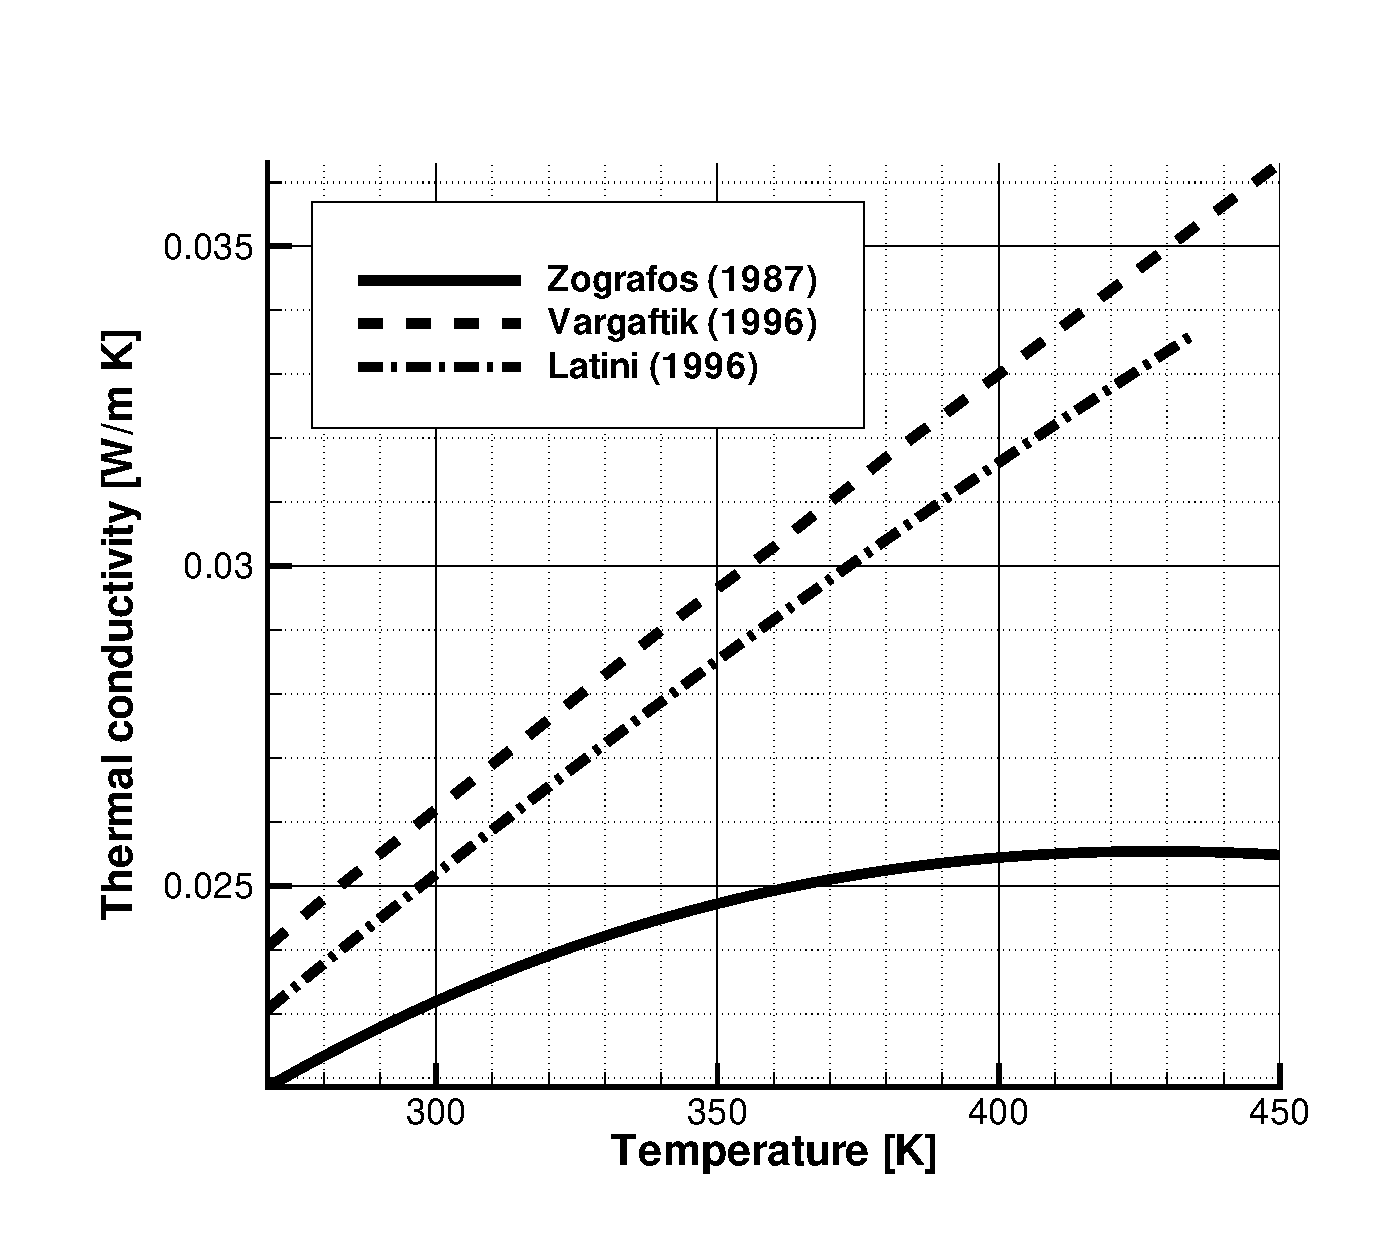
\includegraphics[width=0.49\columnwidth]{chapter20/figures/heat_conductivity_air.eps}
%\centerline{Thermal conductivity}
\end{center}
\caption{Thermal properties of air}
\label{fig:thermal_properties}
\end{figure}
% Mechanical properties
\input{ce_materials_m}
